This section is divided into the approach for the Clean Code Analysis Plattform and the Clean Code classification.

\section{Clean Code Analysis Plattform}
The goal of the design and implementation of the Clean Code Analysis Plattform (CCAP) is a tool for software developers to improve the code quality of existing and new code. The tool accepts a directory containing source code files as input and analyses the input for snippets of improvable code quality. If the analysis classifies a code snippet as problematic, it should help the developer to improve the snippet by providing information about the problem. Ultimately, this should train the developer to spot problematic code by its own and to write clean code by default, so the number of alerts should decrease. At the same time, the overall software quality of a project increases immediately at rewriting a marked snippet and in the long term at training the developer to write code with higher quality.

In order to use the tool effectively, the design and implementation should cover the following requirements:
\begin{description}
    \item[Useability]:  The CCAP should be an easy-to-use tool. Developers shall be able to install and run the tool. The extra effort of using this tool should be small, and the developer should use the tool in his day-to-day workflow without additional friction. The developers can interpret the issue and localise the problematic code spot immediately.
    \item[Expandability]: The extension of the detected code problems should be easy. A clear defined interface for extensions is required so an extension developer would not need specific knowledge about the internal architecture of the tool. The expandability allows the desired workflow of a developer finding problematic code in an, e.g. peer-review, formalising it into an extension and sharing this extension with the team. With each iteration, the code quality of all team members would increase.
    \item[Integration]: The tool should be easy to integrate into different systems. These systems include local workflows like git pre-commits or build systems and remote continuous integration/delivery/deployment pipelines.
\end{description}
A more specific requirement is Python as an input language and the expansion language. After JavaScript, Python is the second most popular programming language 2019 according to the Github statistics (\url{https://octoverse.github.com/#top-languages}). Besides the general popularity, Python is heavily used in the scientific community for machine learning and universities for teaching programming. These groups are part of the potential target audience, and students in specific can benefit from automated reporting of low-quality source code.

\subsection{Architecture}
The CCAP architecture is divided into a static part and two extension possibilities: An extension with analysis plugins adds more rules that are validated by the system. Adding an output plugin allows specifying the output format to fit custom workflow needs.
The static part consists of four components: A core component to act as an orchestration unit, a  component for handling the source code input and a component for handling the analysis plugins as well as output plugins. The design follows the requirements and goals for the platform. 
(TODO: High-level architecture schematic diagram)

The core component contains the main function and handles argument validation and parsing. Furthermore, it orchestrates other components by initialising and executing those. This process is divided into the argument parsing, initialisation and execution phase:
In the argument parsing phase, the command line arguments are parsed and validated. It validates the existence of the required input directory argument and the optional plugin path configuration for the analysis plugins and the output plugins. Additionally, the logging level and the output format can be defined. The latter determines, which output plugin will be used, although the existence of the specified plugin is not validated in this phase. A parsing or validation error will cause a program termination without further processing.
The initialisation phase instantiates all components and the analysis plugin handler will scan the specified directories for plugins and keeps an index of all found plugins in memory. The output plugin manager scans for an output plugin, that satisfies the specified argument. If no plugin matches the output argument, the program will terminate with a one exit code and a failure message to indicate the problem.
In the execution phase, the input handling component scans the input directory for files ending with \textit{.py} and parses the source code into an Abstract Syntax Tree (AST) per file. In the next step, the core passes the parsed data to the analysis plugin handler. The latter will execute all plugins for all files and collects the results. Afterwards, the core component calls the output plugin component to output the results. If no exceptions occur during the execution phase, the program will be terminated with a zero exit code indicating the successful run.

The input component scans the given input directory for all Python source code files and parse the source code into an AST. 
For scanning the input directory, an algorithm will walk recursively over all folders and files. The detection of Python source code files is based on the file ending \textit{.py}. The algorithm will return a list of file paths and the corresponding file content. 
Next, the AST parser is called and will add a parsed AST object to the list besides the file path and content. This list will be passed to the analysis plugins by the analysis plugin handler.  An alternative approach would be to not read and parse the code in the input component, but instead, let the plugins read and parse the file content if needed. With many files to scan, the latter approach would have a lower memory footprint since the file content and the AST will not be held in memory. Consequently, every analysis plugin has to perform an expensive read operation from disk and the performance scales with the number of files and the number of analysis plugins. 
If the input component reads all files, the information is held in the main memory and the performance only scales with the number of files. Since the files are text-based, the number of files needed to exceed the main memory is expected to be high enough to fit most projects. (TODO sample calculation?).

The analysis plugin handler manages all analysis plugins. This component finds all plugins, executes the plugin and collects the reported results.
During the initialisation phase of the core component, the analysis plugin handler will scan the plugin directory for all Python files. It imports all Python files and scans those for classes, that inherit from an abstract \textit{AbstractAnalysisPlugin} class. The abstract class defines all methods that need to be implemented in the concrete plugin subclass. The analysis plugin handler instantiates all found classes.
During the core execution phase, the core receives a list with the file name, file content and the parsed AST. All plugins are called on a specific entry point method that is defined in \textit{AbstractAnalysisPlugin} with the aforementioned list. The plugin will return an instance of \textit{AnalysisReport} with the plugins metadata and a collection of problems. The report is collected for every plugin into an \textit{FullReport}. Additionally, the report contains information about the overall plugin execution time and run arguments. After all plugins have been executed for all files, the analysis plugin handler returns the \textit{FullReport} to the core component.

The last component in the execution chain is the output plugin handler that will pass the \textit{FullReport} to the specified output plugin. It implements the same algorithm as the analysis plugin handler to find all plugins that inherit from \textit{AbstractOutputPlugin}. Instead of keeping track of all plugins, only the plugin that corresponds to the output format argument is instantiated. The output plugin has an entry point as defined in \textit{AbstractOutputPlugin}  that is called with all the collected results.

\subsubsection{Analysis Plugins}\label{sec:analysis_plugins}
Analysis plugins provide the easy extendability of the platform by developers. All users of the tool can expand the set of problems it can detect by implementing a plugin Python and placing it into the plugin directory of the tool. In order to be compatible with the core components, a plugin has to be a class that inherits from the \textit{AbstractAnalysisPlugin} class. Firstly, the abstract class introduces a class member variable \textit{metadata} of the class \textit{PluginMetaData}. A concrete plugin class sets this class member in the constructor to provide a plugin name, author and optional website. This metadata is used in the output to show more information about the plugin that reported a problem. Secondly, \textit{AbstractAnalysisPlugin} specifies a \textit{do\_analysis} method that serves as a entry point that the platform will call. It accepts a list of \textit{ParsedSourceFile} objects that contains the file path, the file content and the corresponding AST for all input files. With this information, the plugin can implement any logic to detect problems. 
For example, the plugin can traverse the AST to look for specific node types, it can use a tokeniser on the content of the files and analyse the token stream or it can run sophisticated machine learning algorithms on the source code.
The plugin can even import third-party libraries, although they have to be installed by the user on the system. After detecting all problems, the plugin returns an \textit{AnalysisReport}. The report contains the plugins metadata and a list of found problems. These problems are instances of a problem class inheriting from \textit{AbstractAnalysisProblem}. The abstract class expects a file path and line number as constructor arguments and requires the plugin developer to override the problem name and description (see listing \ref{lst:lst:return_none_problem_override} for an example). The problem name and description will be shown in the final output and should follow the following guidelines:

\begin{minipage}[c]{0.95\linewidth}

\begin{lstlisting}[language=Python, label=lst:return_none_problem_override, caption={Example for overwriting the \textit{AbstractAnalysisProblem} with a concete implmentation. The problem name and description are overwritten.}]
class ReturnNoneProblem(AbstractAnalysisProblem):
    def __init__(self, file_path, line_number):
        self.name = "Returned None"
        self.description = "Returning None is dangerous since the caller has to check for None. Otherwise, a runtime exception may occur."
        super().__init__(file_path, line_number)
\end{lstlisting}
\end{minipage}

\begin{itemize}
    \item Have a proper name that allows the experienced developer to recognise the problem quickly.
    \item Explain what code construct is problematic.
    \item Give reasons why this code is seen as problematic.
    \item Show guidance and examples on how to fix the problem and improve the code.
\end{itemize}
Although it is possible to use one plugin for multiple, different problem types, having one plugin for one problem type helps to reuse and share the plugin. Additionally, it can be disabled easily by removing the plugin from the plugin folder.

\paragraph{Steps to create an analysis plugin}
In order to expand the CCAP with an analysis plugin, the following steps are required for a developer:
\begin{enumerate}
    \item Create a \textit{.py} file with a class inheriting from \textit{AbstractAnalysisPlugin}.
    \item Instanziate \textit{PluginMetaData} and assign it to the metadata member.
    \item Define a problem class inheriting from \textit{AbstractAnalysisProblem} and set the problem name and description following the guidelines above.
    \item Implement the \textit{do\_analysis} method with a \textit{ParsedSourceFile} parameter. Return an \textit{AnalysisReport} instance with all found problems.
    \item Place the \textit{.py} file into the analysis plugin directory of the tool.
\end{enumerate}
Whereas these are the minimum required steps to implement the plugin, the developer is free to add additional methods, classes or import libraries as necessary.
Furthermore, it is advisable to implement several tests to ensure the plugins correctness. CCAP uses pytest \footnote{\url{https://docs.pytest.org/en/stable/}} for testing, implementing a test is as easy as writing a function with a \enquote{test\_} prefix and running the \textit{pytest} command. The plugin can be tested by simulating a call from the CCAP core with a mocked \textit{ParsedSourceFile}. 

\paragraph{Return None Plugin}
A rather simple analysis plugin demonstrates the capabilities of the CCAP: The Return None Plugin scans the source code for functions that return the None value. Returning None may result in runtime exceptions if the function caller does not expect and handle a potential None return. Although the None can be returned directly or as a value of the returning variable, this plugin only focus on the explicit \textit{return None} statement to showcase the options for the developer to analyse the source code.

Detecting \textit{return None} is possible in multiple ways. The following shows the possibilities for developer to implement such a detector:
\begin{description}
    \item[Regular Expression]: In the \textit{do\_analysis} method, a developer has access to the source code as a string. Therefore, it is straitforward to use a regular expression to detect a \textit{return None} statement.
    \begin{lstlisting}[language=Python]
import re
matches = re.finditer(r"return None", source_file.content, re.MULTILINE | re.DOTALL) \end{lstlisting}
    Since the regex library only returns the start and end index of matches, these have to be converted to line numbers. Afterwards a \textit{ReturnNullProblem} instance can be created for every match and added to the \textit{AnalysisReport} for this plugin.

    This approach uses regular expressions to match patterns in a string without utilising the structures of the code. It is a simple but powerful way and most developers are familiar with regular expression. On the flip-side, source code may have various ways syntactic ways to express a semantic. Consequently, the regular expressions have to be designed carefully to cover all variations. For instance, it is possible to encounter a doubled whitespace, that would break the aforementioned regular expression. Additionally, regular expressions do not operate on the structure of the code; therefore, they can not detect high-level patterns on the code structure.
    \item[Tokenisation]: The process of dividing a character stream into a sequence of tokens is called tokenisation (also known as lexical analysis). With the Python tokeniser, a token can contain multiple characters and has a token type like name, operator or indentation. A token sequence provides more information about the code structure that can be used to detect problematic patterns. 
    A token sequence for a \textit{return None} statement would be the following: 
    \begin{lstlisting}
    [...(type: NAME, value: return), (type: NAME, value: None)...]
    \end{lstlisting}
    A simple algorithm would scan the sequence for two subsequent name tokens with the values "return" and "None". The abstraction level of a token sequence is higher than of a character sequence. Since the whitespace between "return" and "None" provide no semantic meaning, it is removed on this abstraction level. Whereas the regular expression based approach would have to deal with problems as the doubled whitespace, the token-based approach profits from the higher abstraction level and can access meaningful tokens directly.
    \item[Abstract Syntax Tree]: After tokenisation, a parser takes the token stream and prases it into a hierarchical data structure like an Abstract Syntax Tree. With an AST the code is represented structurally and it is possible to traverse the tree following the structure of the code. The AST consists of nodes with different type and children, for example, a node representing an if statement. It is possible to access the condition and the body of the if statement as descendant nodes in the AST. Analysing an AST allows a higher abstraction level then analysing the token string since the code structure is represented. Therefore, more abstract rules that analyse the code structure are possible.

    To detect a \textit{return None} statement in the abstract syntax tree, an algorithm would traverse all AST nodes looking for a return-typed node. If found, the value descendant contains the statement part after the return keyword. A \textit{None} value would be represented as a node of type constant or name constant (depending on the parser version). The value descendant of the constant node may then be checked for equality to \textit{None}. All AST nodes contain the corresponding line number, that are necessary for creating a problem message. See listing \ref{lst:return_none_detection_algorithm} for a Python implementation. 


    Analysing the AST is best for problems in the code structure since the AST represents the code structure in a well-defined, traversable data structure. Although simpler patterns like the \textit{return None} could be detected using regular expressions, a detection on AST level allows detecting the semantic meaning instead of the syntactic representation of a problem. For more complex problems, it is inevitable to use the AST most of the time.
\end{description}

\begin{minipage}[c]{\linewidth}
    \begin{lstlisting}[language=Python, label=lst:return_none_detection_algorithm, caption={Detecting RETURN NONE problems by analsing the AST data structure.}]
    for node in ast.walk(a.ast):
        if isinstance(node, ast.Return):
            return_value = node.value
            if isinstance(return_value, ast.Constant) or isinstance(return_value, ast.NameConstant):
                if return_value.value is None:
                    problems.append(ReturnNullProblem(a.file_path, return_value.lineno))\end{lstlisting}
    \end{minipage}

This implementation covers only the simple case, in which \textit{return None} is written explicitly. Of course, several modifications are possible, that would not be detected by this plugin and would require more sophisticated algorithms. Evaluating, if machine learning models trained on this simple rule can also detect such modifications is part of the second part in research question 3 (TODO: check, jump link).

Since detection alone is not a great help for the user, a useful description of the problem is necessary. 
As described in section \ref{sec:background:returning_none_and_error_handling}, there are some alternatives to returning none. If none happens due to an error, it is better to raise an exception and provoke an explicit error handling, which prevents runtime errors. If the standard return type is a collection, an empty list is more appropriate, since the function caller will most likely write the logic for an unknown amount of list items. However, if the standard return type is a single object, it is not apparent what to return. With PEP484 (TODO source), an optional type was introduced for type hints in Python 3. Using a static type checker for Python like mypy (TODO source) outputs a warning if a developer forgets to check an optional for not being none. 

\paragraph{Condition with Comparison}\label{sec:condition_comparison}
The second plugin detects a direct comparison in a conditional statement. For better readability and understandability, it is suggested to use a function call with an appropriate name that evaluates to true or false. This function call allows a natural reading of the conditional statement without deciphering the meaning of the boolean logic.

An if-statement consists of a condition and body part. If the condition evaluates to true, the body is executed. For the condition, any logical expression will be evaluated. A simple algorithm would take the AST, search for if nodes and check if the condition part is a compare node.
However, negation and logic AND/OR would not be detected by the simple approach. Consequently, a recursive algorithm has to follow logic operators and checks the expressions for comparison nodes. The simple approach does not provide value for the CCAP but we use if for the machine learning evaluation with the problem type name CONDITION COMPARISON SIMPLE.

Following these considerations, an advanced algorithm would scan for if nodes in the AST. The conditional part as a boolean expression is evaluated in a recursive function that returns true if a direct comparison is made anywhere in a boolean expression.
The conditional part can be a boolean operation (like AND/OR) or a unary operator (like NOT).  In these cases, the recursive function will be called again with the respective expressions. If the conditional part is neither a boolean operation nor a unary operator, a true is returned if the conditional part is not a method call. The last case would be the base case in the recursion. Listing \ref{lst:condition_coparison} shows the Python implementation of the recursion.
\begin{minipage}[c]{\linewidth}
\begin{lstlisting}[language=Python, label=lst:condition_coparison, caption={Recursive function to analyse an if statement for direct comparisons. Since a condition should contain a method call, the function returns False if this is not the case.}]
def _check_if_direct_comparison(self, node):
    if isinstance(node, ast.BoolOp):
        violated = False
        #check all expressions of the boolean operator
        for value in node.values:
            if self._check_if_direct_comparison(value):
                violated = True
        return violated
    elif isinstance(node, ast.UnaryOp):
        return self._check_if_direct_comparison(node.operand)

    return not isinstance(node, ast.Call)\end{lstlisting}
\end{minipage}

\subsubsection{Output Plugins}
With output plugins, CCAP adds additional flexibility towards the output format. Depending on environmental requirements, the output can be adapted with custom logic by defining an output plugin. For instance, running the tool locally could write the results to the standard output in a human-readable way or create a formatted HTML file to be displayed in the browser. A machine-readable JSON output may be preferred when running inside an automated workflow.

Output plugins follow similar concepts as analysis plugins. A plugin class inherits from \textit{AbstractOutputPlugin}. The abstract class introduces the metadata member of the \textit{PluginMetaData} class to encapsulate plugin name and author information. Additionally, a second member variable \textit{output\_format} has to be defined with a short abbreviation for the output format. This field is used by the output plugin handler to select the output plugin by the run arguments. Consequently, it should be unique; otherwise, the first found plugin with a matching \textit{output\_format} field is selected by the output plugin handler. Therefore, using a custom prefix string is recommended.

As entry point method, the method \textit{handle\_report} has to be implemented. The method provides an instance of \textit{FullReport} as its argument. The  \textit{report} field holds a collection of  \textit{AnalysisReport} for every analysis plugin that has been executed. With metadata and problem information, the output plugin has access to all required information to produce the desired output.

\paragraph{Steps to create an output plugin}
To expand the output capabilities of the CCAP, the following steps are, similiar to analysis plugins, required:
\begin{enumerate}
    \item Create a \textit{.py} file with a class inheriting from \textit{AbstractOutputPlugin}.
    \item Instanziate \textit{PluginMetaData} and assign it to the metadata member.
    \item Set the \textit{output\_format} field with a unique abbreviation for this output format. Since it should be unique, a custom prefix prevents a name collision with preexisting plugins.
    \item Implement the \textit{handle\_report} method with a \textit{ParsedSourceFile} parameter. 
    \item Place the \textit{.py} file into the output plugin directory of the tool.
\end{enumerate}

\paragraph{Standard Output Plugin}
The Standard Output Plugin writes the formatted output to the stdout stream. It is enabled if no output plugin is explicitly specified. 

The output is divided into a general part and the problem list. The former contains the input path, all executed plugins, a total runtime and a summary field with the numbers of problems in total. The latter displays the list with problems, grouped by analysis plugin.  
For each problem, the problem name, file path, line number and description is printed. A colon separates the file path and line number. Some terminals parse the path and line number so that a user can click the path and it opens the default editor with the cursor in the correct line. Sample output is shown in listing \ref{lst:stdout}.

\begin{minipage}[c]{\linewidth}
\begin{lstlisting}[ columns=fullflexible, label=lst:stdout]
Analysis Report on /Users/d064518/MA_CleanCodeAnalyser/test_programs.
Analyse Plugins: Condition Method Call Plugin, Simple Condition Method Call Plugin, Return None (Null) Plugin, Sample Plugin.
Total time: None
Summary: Found 16 problem(s)
    ----------------------------------------
PROBLEMS:
    PLUGIN NAME: Condition Method Call Plugin by Enrico Kaack <e.kaack@live.de>
        Found: Explicit comparison in condition in /Users/d064518/MA_CleanCodeAnalyser/test_programs/return_none.py:18
            Explicit comparisons in conditions should be replaced by method call for better readability
...
PLUGIN NAME: Return None (Null) Plugin by Enrico Kaack <e.kaack@live.de>
        Found: Returned None in /Users/d064518/MA_CleanCodeAnalyser/test_programs/return_none.py:4
            Returning None is dangerous since the caller has to check for None. Otherwise, a runtime exception may occur.
\end{lstlisting} 
\end{minipage}

\paragraph{HTML Output Plugin}
For larger projects, the Standard Output Plugin may not be sufficient to get an overview of the project or to generate a report. Therefore, the HTML Output Plugin creates a \textit{report.html} file, that can be opened in every browser and provides a cleaner overview. It has similar general data at the top as the Standard Output Plugin, but it moves the problem description into a tooltip to offer a more compact overview. See figure \ref{fig:screen_html_output} for an example screenshot.

\begin{figure}
    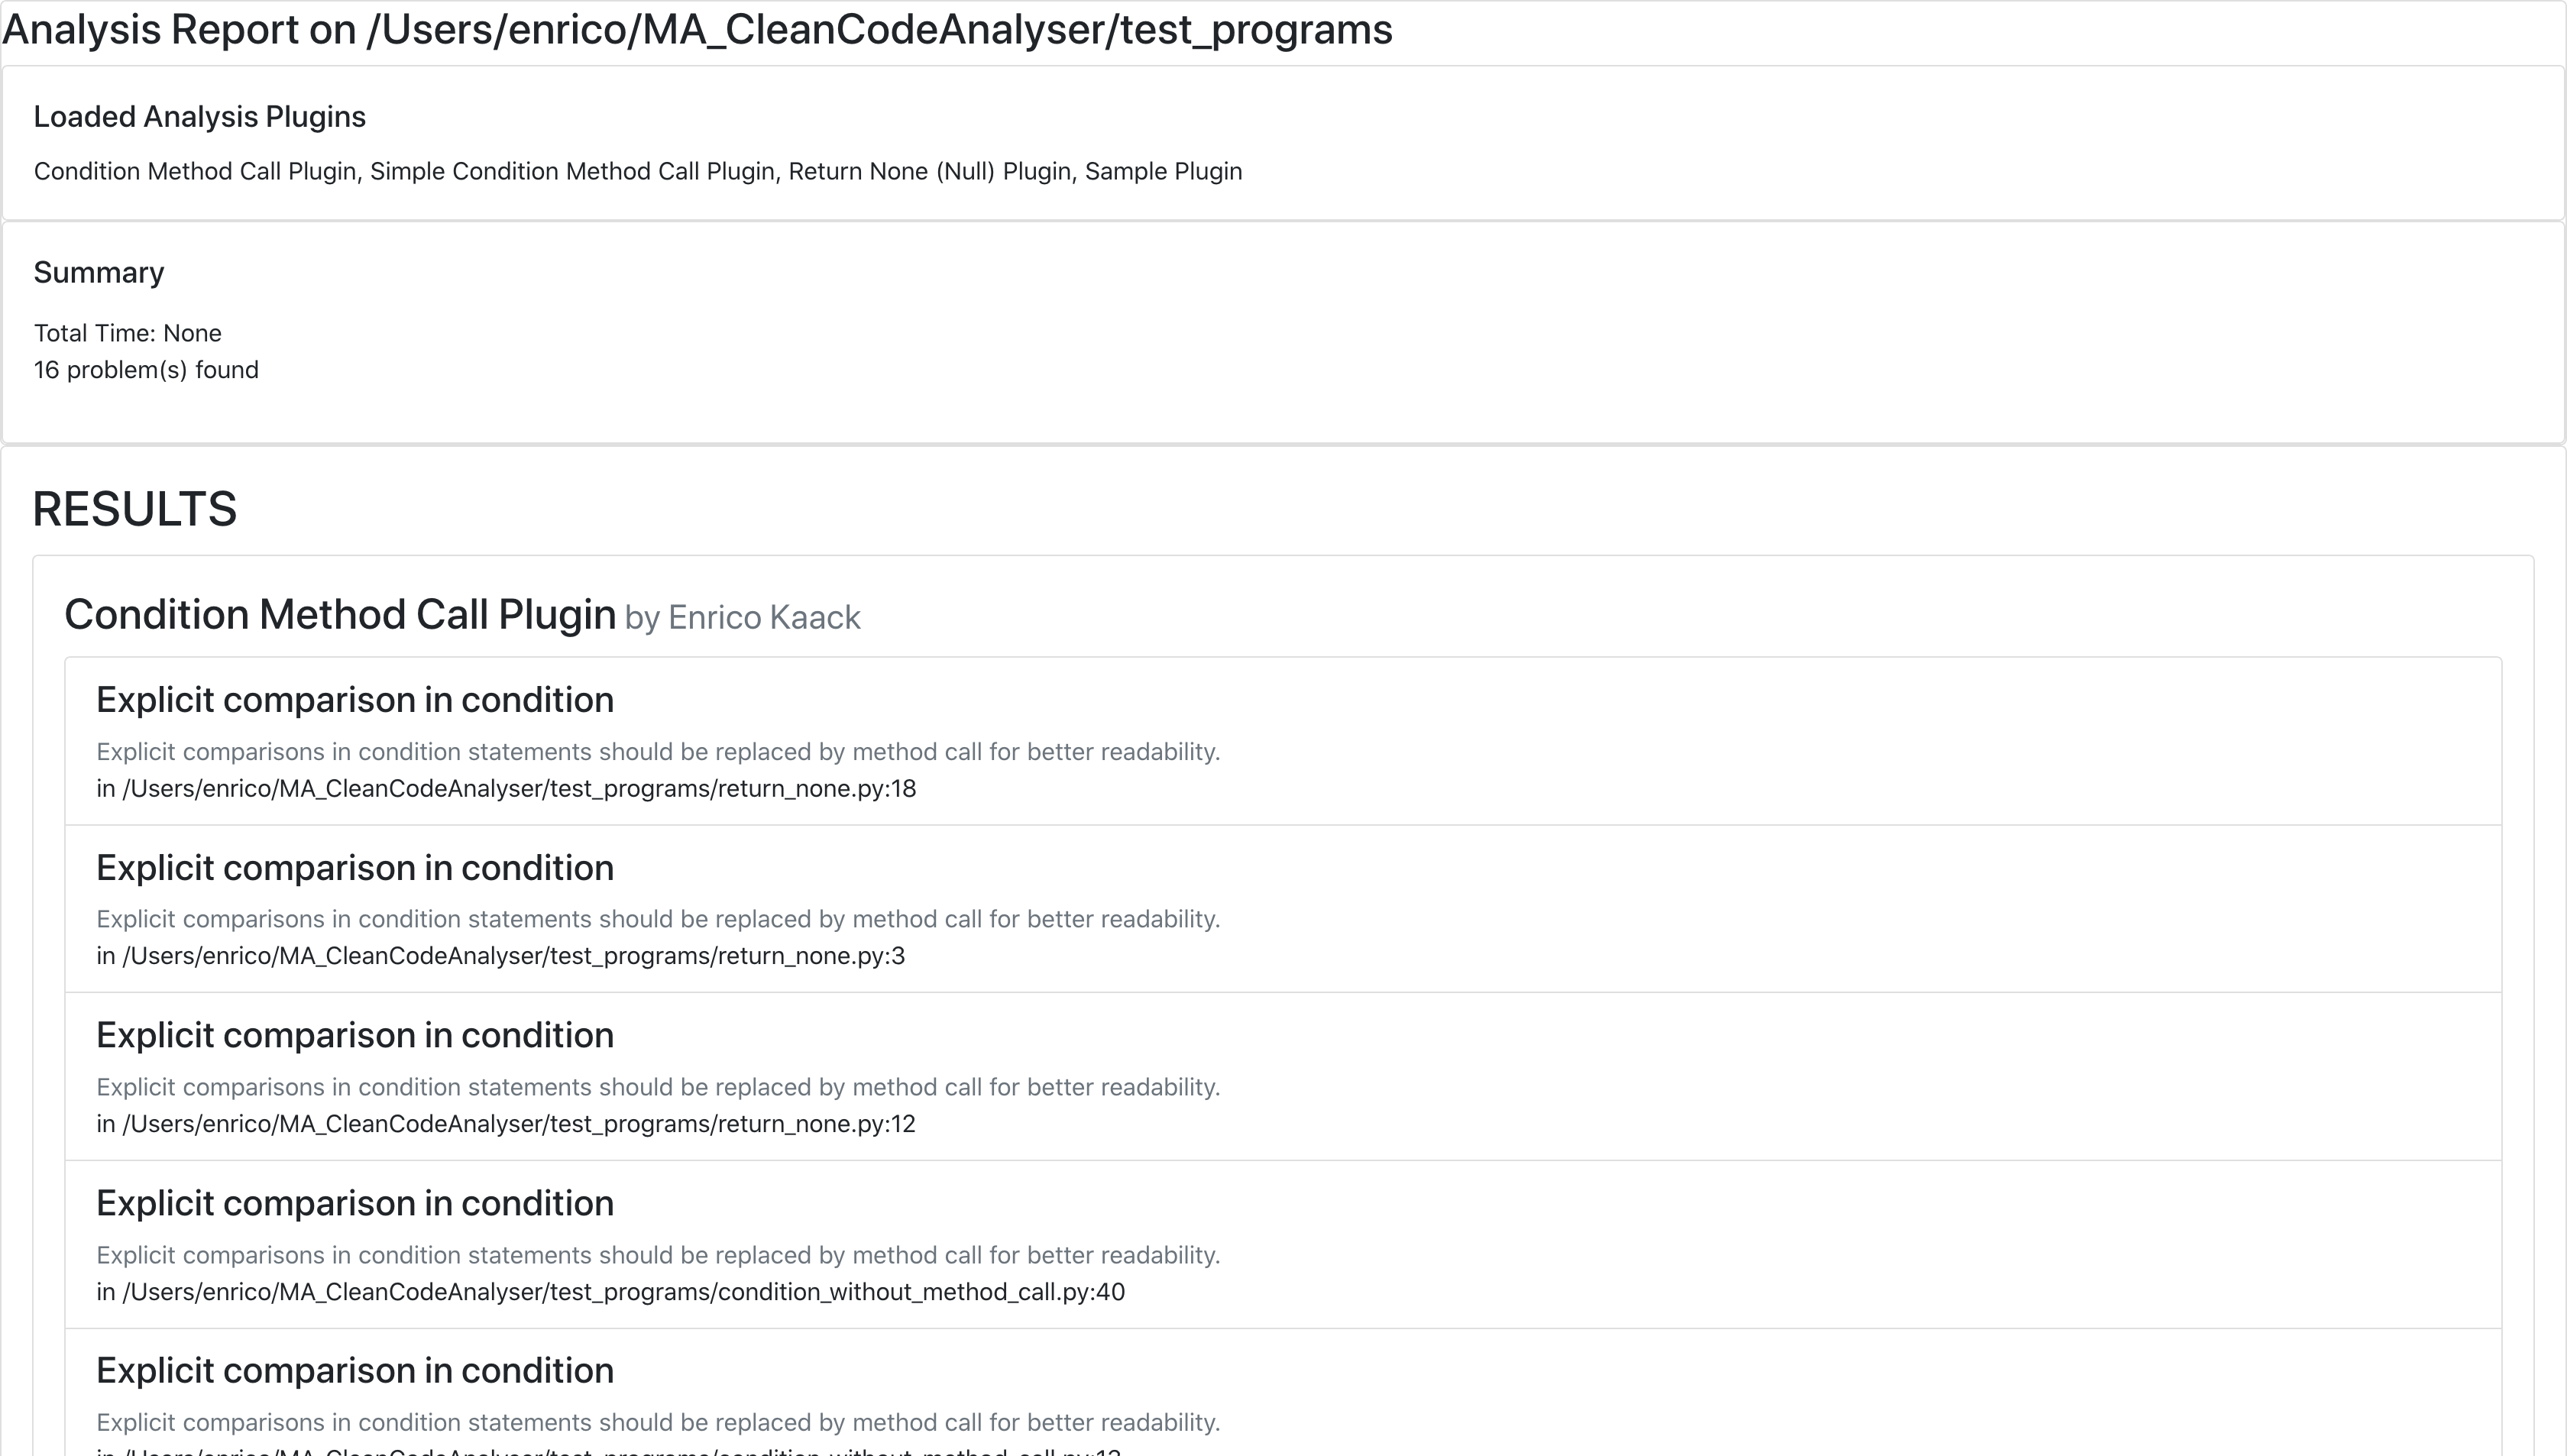
\includegraphics[width=1\textwidth]{img/CCAP/screenshot_html_output.png}
    \label{fig:screen_html_output}
    \caption{Output of the HTML Output Plugin, dispalyed in a browser.}
\end{figure}

\subsection{Extensions}
While the core functionality exists, extensions for the CCAP would aim for improved useability for the user. One important improvement in useability would be an IDE integration for common IDEs like Visual Studio Code. A good starting point would be the Langauge Server Protocol\footnote{\url{https://microsoft.github.io/language-server-protocol/}}. This IDE integration requires a language client as a Visual Studio Code extension and a protocol-compliant language server. The latter would wrap the CCAP and modify it slightly to process a single, changed document and return the results. Since the CCAP architecture is modular, this is possible without larger modifications. 

Another feature would be a configuration to disable specific analysis plugins, that one does not want to run on the project. With the current architecture, this would be possible by moving the analysis plugin file outside the plugin directory. A configuration with command-line parameters or with a per-project, hidden config file would have a better user experience. The latter could also be committed to the version control system, so every team member has the same configuration.
Continuing on configuration possibilities, having configuration possibilities for plugins would increase flexibility for a plugin developer. Introducing configurable warn levels like \enquote*{warning} or \enquote*{error} could help in continuous integration pipelines to decide if a build succeeds but the warnings are reported or if a build should fail because of error-level problems. Some rules could be seen as recommendations (warning level), whereas other rules would be unacceptable (error level).

Lastly, a feature to disable problem reporting for a specific code location could bring a boost in user acceptance. While some clean code rules are objective and can be measured precisely, some rules are more general recommendations that may not apply to every occurrence of this situation. For instance, the clean code guidelines generally suggest not to have more than three function arguments; it may be necessary or even inevitable to have four arguments. The CCAP should report this as a problem, but the user should be able to decide if it is acceptable. In this case, the problem type on this specific location should not be reported in the future. In the current version, the user has no way to ignore a specific problem. Consequently, over time the number of problems the user has to ignore will accumulate until the user abandons the tool since it does not provide an added value over the frustration of manually ignoring problems.

\section{Clean Code Classification}\label{chap:clean_code_classification}
In the previous chapter, we have presented a platform to check for clean code rules. This platform requires analysis plugins to detect certain problems. These handwritten rules work well on certain rules, but certain rules may require a complicated analysis of the AST, the data-flow or the inter-module dependencies. Some rules on the other hand are subjective and we do not see a way of detection those rule violations with an algorithm.
Therefore, this chapter introduces an approach to evaluate different supervised machine learning models to classify code into clean code or problematic code. Furthermore, we describe how we modify the code to test the generalisation capabilities of the models. The mentioned machine learning models include random forest classifier, support-vector-Machines, gradient boosting classifier and a recurrent neural network based on Long short-term memory units. 

The objectives are to train, evaluate and compare Source Code Snippet Classification models and to modify the input data to represent a problematic code in an unseen way.

In the following we describe the approach in detail. The strucutre follows a machine-learning typical pipeline of data collection, preprocessing, encoding, splitting and training. 

\subsection{Challenges}
\paragraph{Lack of datasets}
The most crucial components of every machine learning experiment are labeled datasets. For clean code detection, our research has shown no datasets with labeled clean code violations that could be used.
As a result, we evaluated differnent different appraoches:

\subparagraph{Solution 1:}
Related research fields like code completion often use the py150 (TODO source ) dataset to train models. This dataset contains 150.000 python files, sourced from GitHub. For supervised classification tasks, this dataset is inadequate due to its missing labels.  

\subparagraph{Solution 2:}
Another possible data source would be git commit histories. We could scan the history for commits that fixed unclean code. The previous code could than be labeled \enquote{unclean} and the commited code would be \enquote{clean}.
Same applies to issues and referenced pull requests on GitHub.
We dismissed this approach for several reasons (see figure \ref{fig:commit_messages} for an illustrative example):
\begin{enumerate}
    \item There is no annotation in neither issues descriptions nor git commit messages that would reliably tell, if the change is changing a violation of the clean code rules.
    \item Even if we would be able to find commits that improve chaotic code, we could not ensure automatically, that the commit message is correct and only the improvement is included in the commit.
    \item Searching for commits, we found several clean code improvements and refactorings of large portions of the code base in one commit. Additionally, it is often not explicitly mentioned, which rule applied for the improvement. Consequently, a training with such data could only lead to binary classification into clean code or unclean code. From a practical standpoint, it is advantagous to name the explicit rule violation and to explain how to improve.
\end{enumerate}

\begin{figure}
    \begin{subfigure}{\textwidth}
        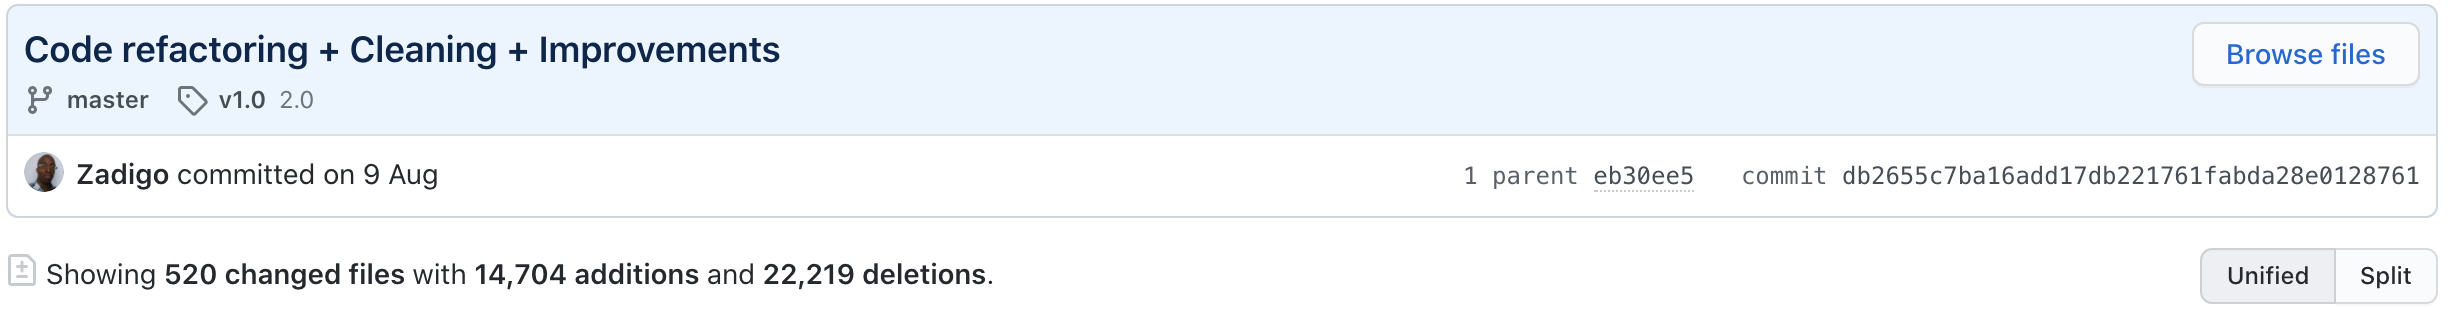
\includegraphics[width=1\linewidth]{img/ML/commit_messages/screen_1.png}
    \end{subfigure}
    \begin{subfigure}{\textwidth}
        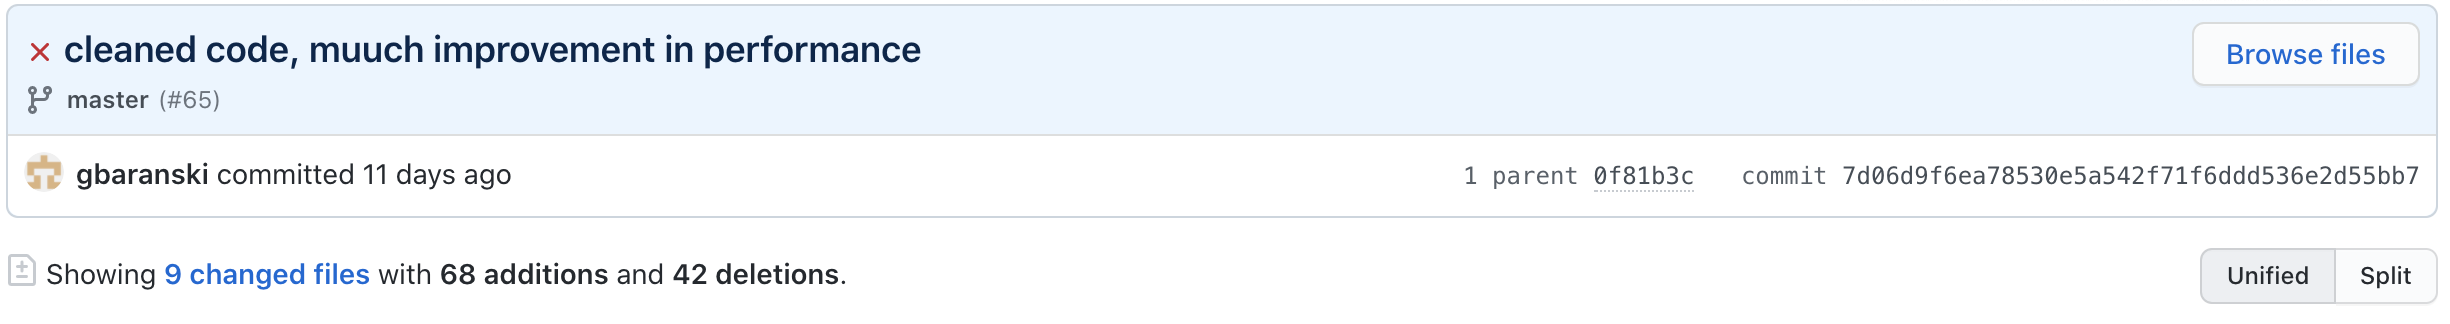
\includegraphics[width=1\linewidth]{img/ML/commit_messages/screen_2.png}
    \end{subfigure}
    \begin{subfigure}{\textwidth}
        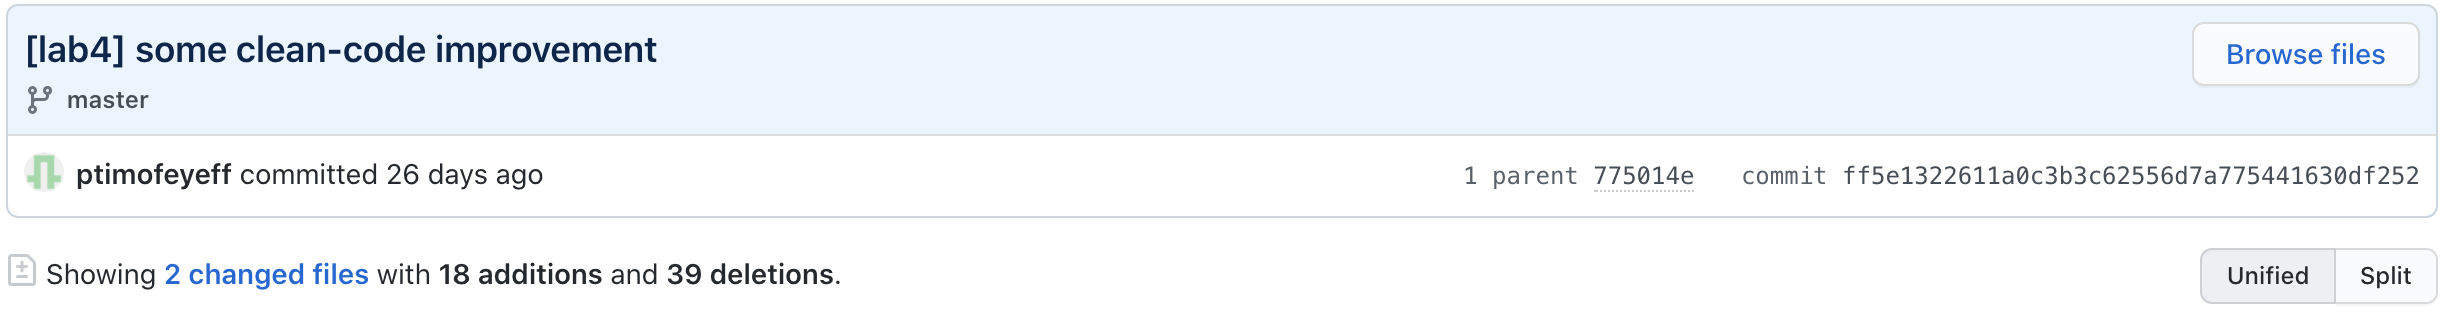
\includegraphics[width=1\linewidth]{img/ML/commit_messages/screen_3.png}
    \end{subfigure}
    \caption[short]%
    {Example commit messages from different repositories. Those examples highlight (1) the missing naming convention, (2) inclusion of additional performance improvements and (3) several edits in multiple files. Those commits are found by searching GitHub for \enquote{clean code improvements} and filtering for Python language and commits. Sources: \footnotemark[1], \footnotemark[2], \footnotemark[3]  }
    \label{fig:commit_messages}
\end{figure}
\footnotetext[1]{\url{https://github.com/Zadigo/ecommerce_template/commit/db2655c7ba16add17db221761fabda28e0128761}}
\footnotetext[2]{\url{https://github.com/gbaranski/homeflow/commit/7d06d9f6ea78530e5a542f71f6ddd536e2d55bb7}}
\footnotetext[3]{\url{https://github.com/ptimofeyeff/distributed-computing/commit/ff5e1322611a0c3b3c62556d7a775441630df252}}
\subparagraph{Solution 3:}
Although Python code is available in abundance in form of open-source projects, it is possible to manually label source code that violates clean code guidelines. 
For the following reasons, we dismissed this approach:
\begin{enumerate}
    \item Curating a hand-labeled dataset is a lot of work that takes time. 
    \item Manual labeling does not ensure correct labeling. A human can make mistakes or can subjectivly misinterpret chaotic code as clean code. The quality of the dataset could suffer and limit the machine learning models performance.
\end{enumerate}
\subparagraph{Solution 4:}
Given any amount of Python files, we could use the analysis plugins from section TODO analysis plugin to reliably detect violations of the corresponding rule. Based on this labeled data, we can train the classifier to detect these rules. If there would be a labeled dataset for more complex clean code rules, we could transfer the findings to these more complex rules. We choose this solution as to solve to solve the dataset problem and train classifier, with more details given in chapter TODO. As a second step, we manipulated the input data, so the original analysis plugin could not detect the still existing problems anymore. With the second step, we show that the classifier generalise well enough to may work on complex clean code rules.

\paragraph{Inbalanced Dataset}\ref{sec:inbalanced_dataset}
A second challenge is a major inbalance between the classes labeled as problematic code and clean code. For the three different problem types, RETURN NONE, CONDITION COMPARISON SIMPLE and CONDITION COMPARISON, the class distribution is shown in table \ref{tab:class_distribution_in_dataset}.



\begin{table}[]
    \begin{tabular}{@{}llll@{}}
    \toprule
    Label  & RETURN NONE & CONDITION SIMPLE & CONDITION COMPARISON \\ \midrule
    0 & 99.79\%     & 97.36\%          & 95.14\%              \\
    1 & 0.21\%      & 2.64\%           & 4.86\%               \\ \bottomrule
    \end{tabular}
    \caption{Class distribution for the train/test dataset before the split. Label [0] represents clean code and label [1] marks problematic code of the corresponding category.}
    \label{tab:class_distribution_in_dataset}
    \end{table}


\subparagraph{Solution 1:}
Due to the inbalance, we do not choose accuracy as a suitable evaluation metric, since classifiying all samples as clean code would result in a accuracy of 99.79\% for the RETURN NONE problem type. Instead, we use precision and recall as metric, with a f1 score as single, weighted metric. More details about the metrics are in chapter TODO.

\subparagraph{Solution 2:}
We will apply undersampling and oversampling techniques on the data and evalaute the difference in model performance. Undersampling removes random samples from the majority class and thus balance class labels. Oversampling replicates random samples from the minority class to balance class labels while also increasing the overall amount of data. This technique is only used on the trainings data. Since it changes the data distribution, an additional train-dev dataset is used as an additional test set to evaluate the impact of the resampling on the model performance. 

\subparagraph{Solution 3:}
Our approach of training different classifier is a solution to the data inbalance, since different classifier have a different sensitivity to data balance. 

\paragraph{SVM quadratic complexity in training}
Support-Vector Machines have a quadratic time complexity on the number of trainings data. Consequently, the training takes a lot of time and the oversampling strategy worsen the trainingstime additionally. 
\subparagraph{Solution:}
We reduced the number of experiments with SVM and just evaluate some simple cases for baseline performance. 

source: 
Time Complexity Analysis of Support Vector Machines
(SVM) in LibSVM

\subsection{Dataset}\label{chap:clean_code_classification_dataset}
The source of our dataset are open-source python projects on GitHub. We queried the top starred python repositories and handselected 18 repositories. Although most top stared repositories are data science frameworks, we additional choose projects from domains such as web server, automation and containerisation. See table TODO for a list of all 18 repositories
A script downlaoded all projects in their main branch with the current head. See table TODO attachment for the corresponding git hashs. Afterwads, we removed all non-python files. 
Next, we uniformly sampled 20\% of all files and seperated those into a holdout set for final testing. 
We ensured to not accidentially change the data distribution on the holdout set. Table \ref{tab:general_data_distribution}, shows general and problem specific metrics for the train/test set and the holdout set. The problem specific metrics are collected after processing the code repositories as described in TODO.

The average lines of code per file is similiar with a small difference of 3.26\%. For all problem types, the difference in lines of code containing the problem is smaller than 0.1 percentage point. This metric is important, since this results in compareable label distribution TODO.
TODO per project analysis table in attachments.

\begin{table}[]
    \begin{tabular}{@{}llll@{}}
        \toprule
    %\cmidrule(l){2-4}
    \multirow{4}{*}{}                            & Metric                  & Train/Test & Holdout \\ \cmidrule(l){2-4} 
                                                 & Lines of Code           & 2,777,268  & 671,554 \\
                                                 & Number of Files         & 14,811     & 3,702   \\
                                                 & average LOC per File    & 187.51     & 181.40     \\ \midrule
    \multirow{2}{*}{Return None}                 & LOCs containing problem & 0.08\%     & 0.08\%  \\
                                                 & Problems per File       & 0.14       & 0.14    \\ \midrule
    \multirow{2}{*}{Condition Comparison Simple} & LOCs containing problem & 1.28\%      & 1.32\%  \\
                                                 & Problems per File       & 2.4       & 2.4    \\ \midrule
    \multirow{2}{*}{Condition Comparison}        & LOCs containing problem & 2.34\%     & 2.44\%  \\
                                                 & Problems per File       & 4.38       & 4.42    \\ \bottomrule
    \end{tabular}
    \caption{General and problem type specific metrics for the Train/Test (before train-test split) and Holdout set. The lines of code containing a problem and the problems per file are similiar.}
    \label{tab:general_data_distribution}
\end{table}

\subsection{Processing}
For the processing steps, we create a pipeline with the d6tflow framework\footnote{\url{https://github.com/d6t/d6tflow}}. Each processing step is a task, that stores its results depending on the parameter configuration in a pickle file. This allows to define a pipeline once and run it with different parameter combinations. The scheduler automatically determines what tasks to run and what task outputs are already stored in pickle files. Consequently, running the pipeline is more efficient and repeatable.

The processing pipeline consists of tasks to read the files into a datastructure, to processes source code and find the problems, to create a vocab dictionary, to convert the data into labeled samples and to split the data into a train, train test and test set. See overview TODO for a schematic representation of the pipeline.

\subsubsection{Files into internal Data Structure}
First, a scanner walks recursively in all subdirectories of the input folder to find all files. If the file has a \textit{.py} extension, its file path and the file content will be stored in a dictionary. The dictionaries for all file are collected into a list. 
Reading all files into main memory increases the performance for downstream tasks, since main memory access is faster than disk access. Although the size of the systems main memory limits the dataset size, a file contains text and is therefore several kilobytes in size. The Train/Test dataset with 14,811 files is 94.98MB in accumulated file size.

\subsubsection{Problem Detection}\label{sec:problem_detection}
As a next step, the analysis plugins from the CCAP (see chapter \ref{sec:analysis_plugins}) process every file and store the line number along with the problem type. As a result, for every file list of problematic line numbers and the corresponding type is available for further processing. The CCAP only covers the two analysis plugins for the problem types CONDITION COMPARISON and RETURN NONE. For model training, we introduce the simple alogrithm to detect comparisons in conditions as problem type CONDITION COMPARISON SIMPLE (described in chapter \ref{sec:condition_comparison})



\subsubsection{Data Encoding}\label{sec:data_encoding}
The data encoding step transform the internal data representation into input vectors x and output vectors y. The transformation is descirbed in the following, multi-stage process.

\paragraph{Fixed Length Sequence}
The length of source code is dynamic, wheras the input size of our models is fixed. Therefore, the character stream of varaible length has to be transformed into a token stream of fixed size. 
To extract meaningful tokens from the character stream, we use the python tokenizer from its standard library. The tokenizer seperates the character stream based on the python syntax definition into tokens. All tokens contain a token type (like a name or operator token), the corresponding characters in the source code and a start and end position (line and column number). Next, the token stream is divided into a fixed size token sequence using a sliding window aproach (size: 20, step size: 3).
\paragraph{Vocabulary Creation}
To represent a token value with a number, every token value needs a numeric representation. Therefore, the occurence of each token value is counted and the index in an descending ordered list for each token value represents the token as an integer. To ignore potential capitalization missmatches, all token values are lower-case. The overall size of the vocabulary is configurable. If the size is smaller than the size of the distinct token value set, the least common token values will be replaced by an unknown token. The unknown token has a numeric representation one bigger than the vocabulary size.
\paragraph{Index-Based Encoding}
The textual token values are encoded with an Index-Based encoding. The most common token values have a numerical representation based on their index in a vocabulary (created with all token values of the train data). Optional, the type of each token is encoded by its numerical representation in the standard library. The type and value encoding are then combined alternating in a final encoding vector that represents an input sample.
\paragraph{Label Extraction}
With the internal representation, the ground truth is encoded as a line number. A transformation is necessary to label each sample corresponding to a given problem type. Label 1 is assigned, if the sample contains the given problem type. A sample contains a problem type, if it contains all tokens from the problematic line. If the sample is missing a token of the problematic line at the beginning or end, the label is 0 for non-problematic code. 

\subsubsection{Train/Test Split}
The data split set is a two-stage process. 
First, the data is split into a train and test set. As discussed in chapter \ref{sec:inbalanced_dataset}, we used over- and undersampling techniques to combat the inbalanced dataset. This is performed solely on the train data. The test data keeps the original distribution. Next, we split the resampled train data into a final train set and a train\_dev set. We use the latter to test the model performance on data with the same distribution as the trainingsdata to additionally evaluate the influence of the data distribution missmatch.

\begin{figure}
    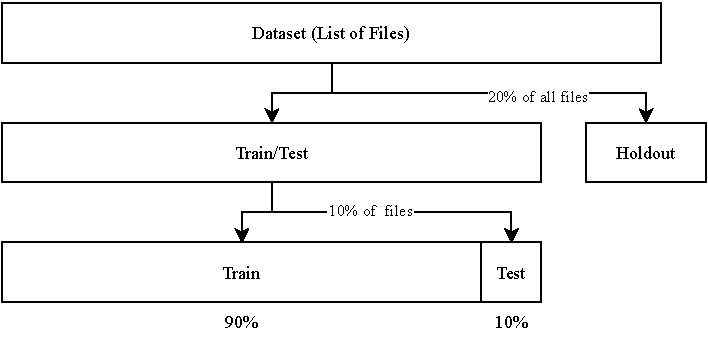
\includegraphics[width=1\textwidth]{img/ML/Data_split.pdf}
    \label{fig:data_split}
    \caption{Split of the dataset. First, 20\% of all files are seperated into a holdout set for later testing. The remainding 80\% of the files are converted samples. The samples are then split again into 70\% training, 10\% train\_dev and 20\% test data. }
\end{figure}

\subsubsection{Models}
Classifying code samples is a binary classification problem since we consider each problem type as a seperate classification task. We train and evaluate a random forest classifier, a support-vector machine based classifier, a gradient boosting classifier and a neural network with LSTM cells.

\paragraph{Random Forest}
We use a random forest classifier with 100 decision trees to perform the binary classification. Additionally to over- and uindersampling, we experiment with an automatic class weighting inverse proportional to class frequency. The other hyperparamter follow the default implementation of the scikit-learn library: The quality measure of a split follows the gini function, the tree depth is unlimited and the number of features to consider for each split is the square-root of the number of features overall.
\paragraph{Support Vector Machine}
\paragraph{Gradient Boosting Classifier}
\paragraph{Neural Networks with LSTM Cells}

\subsubsection{Code Manipulation}
In research question TODO, we evaluate the models generalisation to detect similar pattern the model was not trained on. Therefore, we manipulate the code that it is still a rule violation, but the original analysis plugins would not spot them. 

\paragraph{Return None}\label{par:manipulation_return_none}
For the problem type RETURN NONE, we manipulate the code to have an inline if statement that only returns None in one branch. Therefore, a function may still return None, but the analysis plugin would not detect this. Listing \ref{lst:return_none_modified} shows an example for this case. Although a modification of the analysis plugin could cover the variations as well, we want to see how well machine learning models could perform on this task.

To modify the original code, we use the preprocessed code with problems detected as in chapter \ref{sec:problem_detection}. For every source code line containing the RETURN NONE problem, we use regular expressions to replace the \textit{return None} with a variation as seen in \ref{lst:return_none_modified}. 

The following data encoding step is similiar to the one for model training, although this modified samples will only be used during evaluation.

\begin{minipage}[c]{\linewidth}
\begin{lstlisting}[language=Python, label=lst:return_none_modified, caption={Samples for returning None. The first return would be flagged by the analysis plugin, the second and third return are modified variations that would be ignored by the analysis plugin. The performance of the machine learning models on detecting the latter will be evaluated.}]
def f(a,b):
    #detected by the analysis plugin
    return None 

    #not detected by the analysis plugin
    return None if a < b else b 

    #not detected by the analysis plugin
    return a if a < b else None \end{lstlisting}
\end{minipage}
\paragraph{Condition Comparison}
The analysis for the CONDITION COMPARISON problem type is an advancement of the analysis of the CONDITION COMPARISON SIMPLE problem type.  See listing \ref{lst:conidtion_comparison_modified} for examples of the different analysis results.
Since the results of CONDITION COMPARISON are the modification of the CONDITION COMPARISON SIMPLE, we use the first as ground truth for evaluating the generalisation. Since the CONDITION COMPARISON SIMPLE problems are a subset of the CONDITION COMPARISON problems, we use a similar approach as before (see \ref{par:manipulation_return_none}) to transform all problem occurances to be undectable by the CONDITION COMPARISON SIMPLE analysis plugin.

\begin{minipage}[c]{0.95\linewidth}
\begin{lstlisting}[language=Python, label=lst:conidtion_comparison_modified, caption={Sample statements for the differnce between the two analysis plugins CONDITION COMPARISON and CONDITION COMPARISON SIMPLE.  }]
    def f(a,b):
    #detected by CONDITION COMPARISON SIMPLE
    #detected by CONDITION COMPARISON
    if a < b:
        pass 

    #not detected by CONDITION COMPARISON SIMPLE
    #detected by CONDITION COMPARISON
    if not a < b:
        pass 

    #not detected by CONDITION COMPARISON SIMPLE
    #detected by CONDITION COMPARISON
    if isSmaller(a,b) or a < b:
        pass \end{lstlisting}
\end{minipage}